% !TeX program = xelatex
\documentclass[a4paper,10pt]{article}

% ============================================================================
% សន្លឹកកិច្ចការសិស្ស ស-ខ្មៅ (Student Guided-Inquiry Worksheet - Grade 8 13.2.2 RECT1)
% បរិបទ៖ ថ្នាក់រៀនគ្មានស្លាយ LCD – បំបែកត្រីកោណត្រួតគ្នា និងសម្រាយបញ្ជាក់ ២ ទំព័រ A4
% ============================================================================
\usepackage[a4paper, left=0.90cm, right=0.90cm, top=0.75cm, bottom=0.85cm, footskip=0.45cm]{geometry}
\usepackage{amsmath, amssymb}
\usepackage{unicode-math}
\usepackage{fontspec}
\usepackage{array, colortbl}
\usepackage[table]{xcolor}
\usepackage{enumitem}
\usepackage{pifont}
\usepackage{fancyhdr}
\usepackage{lastpage}
\usepackage{tikz}
\usepackage[most]{tcolorbox}
\usetikzlibrary{calc, arrows.meta, angles, quotes, decorations.markings, positioning, babel}

\makeatletter
\let\@expl@@@mark@update@singlecol@structures@@\relax
\makeatother

\providecommand{\NGSFindFonts}{%
  \IfFileExists{C:/Windows/Fonts/cambria.ttc}{%
    \def\NGSSysPath{C:/Windows/Fonts/}%
    \def\NGSUserPath{C:/Users/KIT/AppData/Local/Microsoft/Windows/Fonts/}%
  }{%
    \IfFileExists{./fonts/KhmerOSsiemreap.ttf}{\def\NGSSysPath{./fonts/}\def\NGSUserPath{./fonts/}}{%
    \IfFileExists{../fonts/KhmerOSsiemreap.ttf}{\def\NGSSysPath{../fonts/}\def\NGSUserPath{../fonts/}}{%
    \IfFileExists{../../fonts/KhmerOSsiemreap.ttf}{\def\NGSSysPath{../../fonts/}\def\NGSUserPath{../../fonts/}}{%
    \IfFileExists{../../../fonts/KhmerOSsiemreap.ttf}{\def\NGSSysPath{../../../fonts/}\def\NGSUserPath{../../../fonts/}}{%
    \IfFileExists{../../../../fonts/KhmerOSsiemreap.ttf}{\def\NGSSysPath{../../../../fonts/}\def\NGSUserPath{../../../../fonts/}}{%
    \IfFileExists{../../../../../fonts/KhmerOSsiemreap.ttf}{\def\NGSSysPath{../../../../../fonts/}\def\NGSUserPath{../../../../../fonts/}}{%
    \IfFileExists{../../../../../../fonts/KhmerOSsiemreap.ttf}{\def\NGSSysPath{../../../../../../fonts/}\def\NGSUserPath{../../../../../../fonts/}}{%
      \def\NGSSysPath{../../../../../../../fonts/}\def\NGSUserPath{../../../../../../../fonts/}%
    }}}}}}}%
  }%
}
\NGSFindFonts

\setmathfont[Path={\NGSSysPath}, FontIndex=1, Scale=1.02]{cambria.ttc}
\defaultfontfeatures{Ligatures=TeX}

\setmainfont[
  Path={\NGSUserPath},
  Extension=.ttf,
  Script=Khmer,
  BoldFont={KhmerOSsiemreap},
  BoldFeatures={FakeBold=1.8},
  ItalicFont={KhmerOSsiemreap},
  ItalicFeatures={FakeSlant=0.25},
  BoldItalicFont={KhmerOSsiemreap},
  BoldItalicFeatures={FakeBold=1.8, FakeSlant=0.25}
]{KhmerOSsiemreap}

\newfontfamily\muol[Path={\NGSUserPath}, Extension=.ttf, Script=Khmer]{KhmerOSmuollight}
\newfontfamily\TimesEn[Path={\NGSSysPath}, Extension=.ttf, BoldFont={timesbd}, ItalicFont={timesi}, BoldItalicFont={timesbi}]{times}

\XeTeXlinebreaklocale "km"
\XeTeXlinebreakskip = 0pt plus 1pt minus 0.1pt

\definecolor{panelgray}{gray}{0.94}
\definecolor{headgray}{gray}{0.86}
\definecolor{subgray}{gray}{0.91}

\pagestyle{fancy}
\fancyhf{}
\renewcommand{\headrulewidth}{0pt}
\fancyfoot[L]{\fontsize{8pt}{10pt}\selectfont អនុវិទ្យាល័យព្រះក្រសាំង \en{|} គណិតវិទ្យា ថ្នាក់ទី៨ \en{|} មេរៀនទី១៣ (២.២ លក្ខណៈចតុកោណកែង)}
\fancyfoot[R]{\fontsize{8.2pt}{10pt}\selectfont ទំព័រ \en{\thepage\ / \pageref{LastPage}}}

\setlength{\parindent}{0pt}
\setlength{\parskip}{0pt}
\setlength{\tabcolsep}{4pt}

\newcommand{\en}[1]{{\TimesEn #1}}
\newcommand{\enbf}[1]{{\TimesEn\textbf{#1}}}
\newcommand{\unit}[1]{\,\text{\en{#1}}}
\newcommand{\cnum}[1]{{\fontsize{10pt}{12pt}\selectfont\ding{\numexpr171+#1\relax}}}
\newcommand{\chk}{\tikz[baseline=-0.15ex]\draw[black, line width=0.8pt] (0,0) rectangle (0.25cm,0.25cm);}
\newcommand{\tri}[1]{\ensuremath{\triangle #1}}
\newcommand{\ang}[1]{\ensuremath{\angle #1}}
\newcommand{\cg}{\ensuremath{\cong}}
\newcommand{\dotline}[1]{\makebox[#1]{\dotfill}}

\newcolumntype{L}[1]{>{\raggedright\arraybackslash}p{#1}}
\newcolumntype{C}[1]{>{\centering\arraybackslash}p{#1}}

\tikzset{
  tk1/.style={postaction={decorate},decoration={markings,mark=at position 0.50 with {\draw[black, line width=0.90pt](0,-0.095)--(0,0.095);}}},
  tk2/.style={postaction={decorate},decoration={markings,
    mark=at position 0.45 with {\draw[black, line width=0.90pt](0,-0.095)--(0,0.095);},
    mark=at position 0.55 with {\draw[black, line width=0.90pt](0,-0.095)--(0,0.095);}}},
  par1/.style={postaction={decorate},decoration={markings,mark=at position 0.52 with {\draw[black, line width=0.90pt](-0.07,0.08)--(0.05,0)--(-0.07,-0.08);}}}
}

\newcommand{\secbar}[2]{%
  \vspace{3pt}
  \noindent\colorbox{headgray}{\parbox{\dimexpr\linewidth-2\fboxsep\relax}{%
    \vspace{1.5pt}{\muol\fontsize{9.5pt}{13.5pt}\selectfont #1}\hfill{\fontsize{8.5pt}{12pt}\selectfont\textbf{#2}}\vspace{1.5pt}%
  }}\par\vspace{3pt}
}

\begin{document}
\fontsize{9.5pt}{14.3pt}\selectfont

% ============================================================================
% ទំព័រទី១៖ E1 ទស្សន៍ទាយ + E2 វាស់ខ្នាតពិត 1:1 & បំបែកត្រីកោណត្រួតគ្នា (Duval Deconstruction)
% ============================================================================
\begin{tcolorbox}[enhanced, sharp corners, colback=white, colframe=black, boxrule=1.0pt, top=4pt, bottom=4pt, left=6pt, right=6pt]
  \begin{center}
    {\muol\fontsize{10.5pt}{15pt}\selectfont សន្លឹកកិច្ចការសិស្ស — មេរៀនទី១៣៖ ចតុកោណ \enbf{(}២.២ លក្ខណៈចតុកោណកែង\enbf{)}}\\[2pt]
    {\footnotesize សៀវភៅសិក្សាគោលថ្នាក់ទី៨ ទំព័រ ១៧៤--១៧៦ និង ១៨៦ \en{|} បំបែកត្រីកោណត្រួតគ្នា និងសម្រាយបញ្ជាក់ (គ្មានស្លាយ \en{LCD})}
  \end{center}
  \vspace{2pt}
  \hrule height 0.5pt
  \vspace{4pt}
  ឈ្មោះសិស្សទី១៖ \dotline{3.6cm} \hspace{0.15cm} ឈ្មោះដៃគូទី២៖ \dotline{3.6cm} \hspace{0.15cm} ថ្នាក់ទី៨៖ \dotline{1.0cm} \hspace{0.15cm} ថ្ងៃទី១៥/១២/២០២៦
\end{tcolorbox}

% --- E1 Engage ---
\secbar{ផ្នែកទី១ ៖ បេសកកម្មផ្ដើមមេរៀន — វិធីផ្ទៀងជ្រុងកែងស៊ុមបង្អួចដោយខ្សែពួរ \enbf{(E1 -- Engage)}}{៣ នាទី}
\begin{tcolorbox}[enhanced, sharp corners, colback=panelgray, colframe=black, boxrule=0.7pt, top=3.5pt, bottom=3.5pt, left=6pt, right=6pt]
  \textbf{ស្ថានភាពពិត៖} ជាងឈើដំឡើងស៊ុមបង្អួច $ABCD$ ដោយកាត់ឈើឈមប្រវែងស្មើគ្នា ($AB=CD$ និង $AD=BC$) តែភ្លេចយកដែកកែងមក ។ គាត់យកខ្សែពួរវាស់ប្រៀបធៀបតែអង្កត់ទ្រូង $AC$ និង $BD$ ប៉ុណ្ណោះ!\par\vspace{1.5pt}
  $\bullet$ \textbf{មេជាង ក ថា៖} «ឱ្យតែខ្សែទ្រូង $AC = BD$ ស៊ុមបង្អួចនេះច្បាស់ជាកែងជ្រុងទាំង ៤ ($90^\circ$) ១០០\%!»\par
  $\bullet$ \textbf{កូនជាង ខ ឆ្ងល់ថា៖} «ចុះចតុកោណព្នាយសមបាតក៏មានអង្កត់ទ្រូងស្មើគ្នាដែរ ហេតុអ្វីមុំរបស់វាមិនកែង?»\par\vspace{1.5pt}
  \textbf{ការទស្សន៍ទាយដំបូងរបស់ដៃគូអ្នក៖} \hspace{0.3cm} \chk\ មេជាង ក ត្រូវ \hspace{0.6cm} \chk\ កូនជាង ខ ត្រូវ \hspace{0.6cm} \chk\ មិនទាន់ប្រាកដ
\end{tcolorbox}

% --- E2 Explore ---
\secbar{ផ្នែកទី២ ៖ វាស់ខ្នាតពិត \enbf{1:1} និងបំបែកត្រីកោណត្រួតគ្នា \enbf{(E2 -- Explore)}}{១១ នាទី}
\textbf{សកម្មភាពទី១ (៥ នាទី)៖} ប្រើបន្ទាត់ក្រិត និងរ៉ាប់ព័រទ័រ វាស់ចតុកោណកែងខ្នាតពិត $ABCD$ ($4.0\unit{cm}\times 3.0\unit{cm}$) ខាងឆ្វេង រួចបំពេញតារាង៖\par\vspace{3pt}
\begin{tabular}{@{}C{6.40cm} L{12.20cm}@{}}
  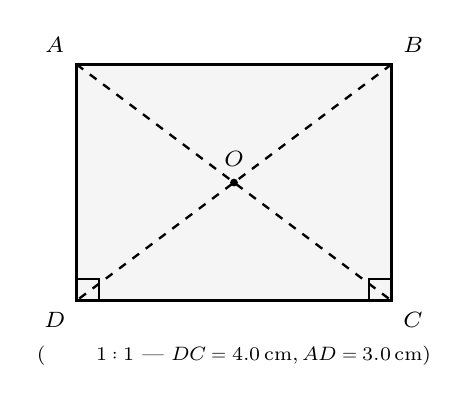
\begin{tikzpicture}[x=1cm, y=1cm, baseline={(0,1.75)}, every node/.style={font=\footnotesize, text=black}]
    \coordinate (D) at (0,0);
    \coordinate (C) at (4.0,0);
    \coordinate (A) at (0,3.0);
    \coordinate (B) at (4.0,3.0);
    \coordinate (O) at (2.0,1.5);
    \fill[gray!8] (A)--(B)--(C)--(D)--cycle;
    \draw[black, line width=1.05pt] (A)--(B)--(C)--(D)--cycle;
    \draw[black, line width=0.85pt, dashed] (A)--(C) (B)--(D);
    \draw[black, line width=0.7pt] (0,0.28)--(0.28,0.28)--(0.28,0);
    \draw[black, line width=0.7pt] (3.72,0)--(3.72,0.28)--(4.0,0.28);
    \fill[black] (O) circle (1.4pt) node[above=2pt] {$O$};
    \node[above left=1pt] at (A) {$A$};
    \node[above right=1pt] at (B) {$B$};
    \node[below right=1pt] at (C) {$C$};
    \node[below left=1pt] at (D) {$D$};
    \node[anchor=north, font=\scriptsize] at (2.0,-0.45) {(ខ្នាតពិត $1:1$ — $DC=4.0\unit{cm}, AD=3.0\unit{cm}$)};
  \end{tikzpicture}
  &
  {\renewcommand{\arraystretch}{1.26}
  \begin{tabular}{|L{4.85cm}|L{6.55cm}|}
    \hline
    \rowcolor{subgray}\textbf{ធាតុដែលត្រូវវាស់} & \textbf{លទ្ធផលវាស់ និងការសង្កេត} \\
    \hline
    អង្កត់ទ្រូងពេញ $AC$ និង $BD$ & $AC = \dotline{1.4cm}\unit{cm}$, $BD = \dotline{1.4cm}\unit{cm}$ (\chk\ ស្មើ) \\
    \hline
    កំណាត់ពីផ្ចិត $O$ ទាំងបួន & $OA=\dotline{1.0cm}$, $OB=\dotline{1.0cm}$, $OC=\dotline{1.0cm}$, $OD=\dotline{1.0cm}$ \\
    \hline
    ប្រភេទនៃ $\tri{OAB}$ និង $\tri{OAD}$ & ជាត្រីកោណ \dotline{3.8cm} \\
    \hline
    \textbf{អន្ទាក់មុំពុះ៖} វាស់ $\ang{DAC}$ និង $\ang{CAB}$ & $\ang{DAC}\approx\dotline{1.1cm}^\circ$, $\ang{CAB}\approx\dotline{1.1cm}^\circ$ (\chk\ ស្មើ $45^\circ$ \chk\ មិនស្មើ) \\
    \hline
    ហេតុអ្វីចតុកោណព្នាយសមបាតមាន $EG=FH$ តែមុំមិនកែង? & ព្រោះចតុកោណព្នាយសមបាត \textbf{មិនមែនជា} \dotline{2.2cm} (ជ្រុងឈមមិនស្របគ្នាទាំងពីរគូទេ!) \\
    \hline
  \end{tabular}}
\end{tabular}

\vspace{4pt}
\textbf{សកម្មភាពទី២ — បំបែកត្រីកោណត្រួតគ្នា $\tri{ADC}$ និង $\tri{BDC}$ (\en{Duval Deconstruction}, ៦ នាទី)៖} គូស \textbf{[tracing]} ព័ទ្ធជ្រុងរួម $DC$ រួចបំពេញ៖\par\vspace{2pt}
{\renewcommand{\arraystretch}{1.18}
\begin{tabular}{|L{9.15cm}|L{9.15cm}|}
  \hline
  \rowcolor{subgray}\textbf{ផ្នែក ក៖ ទ្រឹស្ដីបទទី២ ($ABCD$ ចតុកោណកែង $\Rightarrow AC=BD$)} & \textbf{ផ្នែក ខ៖ ទ្រឹស្ដីបទទី៣ (ប្រលេឡូក្រាមមាន $AC=BD \Rightarrow$ កែង)} \\
  \hline
  \begin{center}
  \vspace{-2pt}
  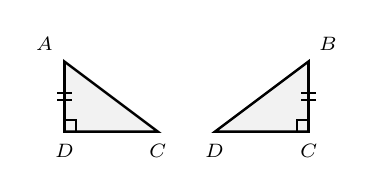
\begin{tikzpicture}[scale=0.66, every node/.style={font=\scriptsize}]
    % \triangle ADC
    \draw[line width=0.9pt, fill=gray!10] (0,0)--(1.8,0)--(0,1.35)--cycle;
    \draw[line width=0.9pt, tk2] (0,0)--(0,1.35);
    \draw[line width=0.65pt] (0,0.22)--(0.22,0.22)--(0.22,0);
    \node[above left=0.5pt] at (0,1.35) {$A$}; \node[below=1pt] at (0,0) {$D$}; \node[below=1pt] at (1.8,0) {$C$};
    % \triangle BDC
    \begin{scope}[shift={(2.90,0)}]
      \draw[line width=0.9pt, fill=gray!10] (0,0)--(1.8,0)--(1.8,1.35)--cycle;
      \draw[line width=0.9pt, tk2] (1.8,0)--(1.8,1.35);
      \draw[line width=0.65pt] (1.58,0)--(1.58,0.22)--(1.8,0.22);
      \node[above right=0.5pt] at (1.8,1.35) {$B$}; \node[below=1pt] at (0,0) {$D$}; \node[below=1pt] at (1.8,0) {$C$};
    \end{scope}
  \end{tikzpicture}
  \vspace{-3pt}
  \end{center}
  បំបែក $\tri{ADC}$ និង $\tri{BDC}$ ដាច់ពីគ្នា មាន៖\par
  ១. ជ្រុង $AD = \dotline{1.2cm}$ (ជ្រុងឈមនៃចតុកោណកែង)\par
  ២. មុំ $\ang{ADC} = \ang{\dotline{1.2cm}} = 90^\circ$ (មុំកែង)\par
  ៣. ជ្រុង $DC$ ជាជ្រុង \dotline{1.5cm} (\textbf{[tracing]})\par
  $\Rightarrow \tri{ADC} \cg \tri{BDC}$ តាមលក្ខណៈ (\dotline{1.4cm})\par
  $\bullet$ \textbf{សន្និដ្ឋាន៖} អង្កត់ទ្រូង $AC = \dotline{1.5cm}$ ។
  &
  \begin{center}
  \vspace{-2pt}
  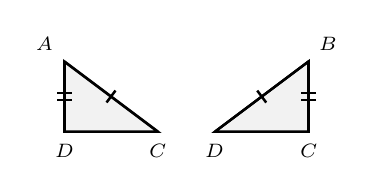
\begin{tikzpicture}[scale=0.66, every node/.style={font=\scriptsize}]
    % \triangle ADC
    \draw[line width=0.9pt, fill=gray!10] (0,0)--(1.8,0)--(0,1.35)--cycle;
    \draw[line width=0.9pt, tk2] (0,0)--(0,1.35);
    \draw[line width=0.9pt, tk1] (0,1.35)--(1.8,0);
    \node[above left=0.5pt] at (0,1.35) {$A$}; \node[below=1pt] at (0,0) {$D$}; \node[below=1pt] at (1.8,0) {$C$};
    % \triangle BDC
    \begin{scope}[shift={(2.90,0)}]
      \draw[line width=0.9pt, fill=gray!10] (0,0)--(1.8,0)--(1.8,1.35)--cycle;
      \draw[line width=0.9pt, tk2] (1.8,0)--(1.8,1.35);
      \draw[line width=0.9pt, tk1] (0,0)--(1.8,1.35);
      \node[above right=0.5pt] at (1.8,1.35) {$B$}; \node[below=1pt] at (0,0) {$D$}; \node[below=1pt] at (1.8,0) {$C$};
    \end{scope}
  \end{tikzpicture}
  \vspace{-3pt}
  \end{center}
  ក្នុងប្រលេឡូក្រាម $ABCD$ ដែលមាន $AC = BD$៖\par
  ១. $AD = \dotline{1.1cm}$ (ជ្រុងឈមប្រលេឡូក្រាម)\par
  ២. $AC = \dotline{1.1cm}$ (សម្មតិកម្ម) និង $DC$ ជាជ្រុង \dotline{1.4cm}\par
  $\Rightarrow \tri{ADC} \cg \tri{BDC}$ តាមលក្ខណៈ (\dotline{1.4cm}) $\Rightarrow \ang{ADC}=\ang{\dotline{1.1cm}}$\par
  $\bullet$ តែ $\ang{ADC}+\ang{BCD} = 180^\circ \Rightarrow 2\ang{BCD}=180^\circ \Rightarrow \ang{BCD}=\dotline{0.9cm}^\circ$\par
  $\bullet$ \textbf{សន្និដ្ឋាន៖} $ABCD$ ជា \dotline{2.6cm} ។ \\
  \hline
\end{tabular}}

\newpage

% ============================================================================
% ទំព័រទី២៖ E3 ធនាគារហេតុផល ①–⑤ + E4 លំហាត់គំរូ ២ + E5 ប្រតិបត្តិ & Exit Check + កិច្ចការផ្ទះ
% ============================================================================
\secbar{ផ្នែកទី៣ ៖ សង្ខេបលក្ខណៈចតុកោណកែង និងធនាគារហេតុផល \cnum{1}--\cnum{5} \enbf{(E3 -- Explain)}}{៦ នាទី}
\begin{tcolorbox}[enhanced, sharp corners, colback=white, colframe=black, boxrule=0.8pt, top=3.5pt, bottom=3.5pt, left=6pt, right=6pt]
  \cnum{1} \textbf{និយមន័យ៖} ចតុកោណកែង ជា \dotline{2.6cm} ដែលមានមុំកែងមួយ (មានគ្រប់លក្ខណៈរបស់ប្រលេឡូក្រាម) ។\par\vspace{1.5pt}
  \cnum{2} \textbf{ទ្រឹស្ដីបទទី១៖} មុំទាំងបួននៃចតុកោណកែងសុទ្ធតែជាមុំ \dotline{2.0cm} ($\ang{A}=\ang{B}=\ang{C}=\ang{D}=90^\circ$) ។\par\vspace{1.5pt}
  \cnum{3} \textbf{ទ្រឹស្ដីបទទី២៖} អង្កត់ទ្រូងទាំងពីរនៃចតុកោណកែង \dotline{2.2cm} ($AC = BD$) ។\par\vspace{1.5pt}
  \cnum{4} \textbf{វិបាកអង្កត់ទ្រូង៖} កំណាត់អង្កត់ទ្រូងទាំងបួនស្មើគ្នា ($OA = OB = OC = OD = \frac{1}{2}\dotline{1.0cm}$) ។\par\vspace{1.5pt}
  \cnum{5} \textbf{ទ្រឹស្ដីបទទី៣ (សម្គាល់)៖} ប្រលេឡូក្រាមដែលមានអង្កត់ទ្រូង \dotline{2.0cm} ជាចតុកោណកែង (ឬចតុកោណមានមុំកែង ៣) ។
\end{tcolorbox}

% --- E4 Elaborate ---
\secbar{ផ្នែកទី៤ ៖ លំហាត់គំរូអនុវត្ត \enbf{[tracing]} និងធនាគារហេតុផល \cnum{1}--\cnum{5} \enbf{(E4 -- Elaborate)}}{១០ នាទី}
{\renewcommand{\arraystretch}{1.20}
\begin{tabular}{|L{9.15cm}|L{9.15cm}|}
  \hline
  \rowcolor{subgray}\textbf{គំរូទី១ (លំហាត់ទី៩ ទំ.១៨៦ — ភ្ជាប់តាមអង្កត់ទ្រូង $BE$)} & \textbf{គំរូទី២ (លំហាត់គំរូ ទំ.១៧៦ — ផលបូកចម្ងាយកែង $MP+MQ=BH$)} \\
  \hline
  គេមានចតុកោណកែង $ABCE$ និងប្រលេឡូក្រាម $BCDE$ ។ បង្ហាញថាត្រីកោណ $ACD$ ជាត្រីកោណសមបាត ។\par
  \begin{center}
  \vspace{-2pt}
  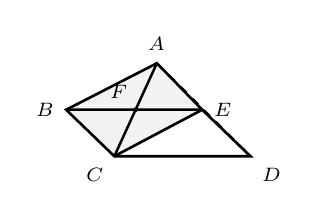
\begin{tikzpicture}[scale=0.72, every node/.style={font=\scriptsize}]
    \coordinate (C) at (0.85,0); \coordinate (D) at (3.25,0);
    \coordinate (B) at (0,0.82); \coordinate (E) at (2.40,0.82);
    \coordinate (A) at (1.60,1.64); \coordinate (F) at ($(A)!0.5!(C)$);
    \fill[gray!10] (A)--(B)--(C)--(E)--cycle;
    \draw[line width=0.95pt] (A)--(B)--(C)--(E)--cycle;
    \draw[line width=0.95pt] (C)--(D)--(E);
    \draw[line width=0.9pt] (A)--(C) (B)--(E);
    \draw[line width=0.8pt, dashed] (A)--(D);
    \fill (F) circle (1.2pt) node[above left=0.5pt] {$F$};
    \node[above=1pt] at (A) {$A$}; \node[left=1pt] at (B) {$B$};
    \node[below left=1pt] at (C) {$C$}; \node[below right=1pt] at (D) {$D$}; \node[right=1pt] at (E) {$E$};
  \end{tikzpicture}
  \vspace{-2pt}
  \end{center}
  $\bullet$ ក្នុងចតុកោណកែង $ABCE$៖ អង្កត់ទ្រូង $AC = \dotline{1.0cm}$ (តាម \cnum{3})\par
  $\bullet$ ក្នុងប្រលេឡូក្រាម $BCDE$៖ ជ្រុងឈម $BE = \dotline{1.0cm}$\par
  $\bullet$ តាមលក្ខណៈឆ្លង៖ គេបាន $AC = \dotline{1.0cm}$\par
  $\bullet$ ដូច្នេះ $\tri{ACD}$ ជាត្រីកោណ \dotline{2.1cm} កំពូល \dotline{0.7cm} ។
  &
  ត្រីកោណសមបាត $ABC$ ($AB=AC$), $M\in BC$, $MP\perp AB, MQ\perp AC$ ។ បន្លាយ $QM$ ឱ្យបាន $MR=MP$, $BH\perp AC$ ។ បង្ហាញថា $MP+MQ=BH$ ។\par
  \begin{center}
  \vspace{-3pt}
  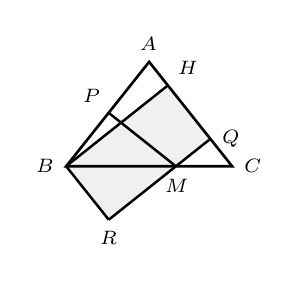
\begin{tikzpicture}[scale=0.68, every node/.style={font=\scriptsize}]
    \coordinate (B) at (0,0); \coordinate (C) at (3.1,0); \coordinate (A) at (1.55,1.95);
    \coordinate (M) at (2.05,0);
    \coordinate (P) at ($(A)!(M)!(B)$); \coordinate (Q) at ($(A)!(M)!(C)$); \coordinate (H) at ($(A)!(B)!(C)$);
    \path let \p1 = ($(M)-(P)$), \p2 = ($(M)-(Q)$), \n1 = {veclen(\x1,\y1)}, \n2 = {veclen(\x2,\y2)} in
          coordinate (R) at ($(M) + {\n1/\n2}*($(M)-(Q)$)$);
    \fill[gray!12] (B)--(H)--(Q)--(R)--cycle;
    \draw[line width=0.95pt] (A)--(B)--(C)--cycle;
    \draw[line width=0.9pt] (B)--(H) (M)--(P) (Q)--(R) (B)--(R);
    \node[above=0.5pt] at (A) {$A$}; \node[left=1pt] at (B) {$B$}; \node[right=1pt] at (C) {$C$};
    \node[above left=0.5pt] at (P) {$P$}; \node[above right=0.5pt] at (H) {$H$};
    \node[right=1pt] at (Q) {$Q$}; \node[below=1pt] at (M) {$M$}; \node[below=0.5pt] at (R) {$R$};
  \end{tikzpicture}
  \vspace{-2pt}
  \end{center}
  $\bullet$ មុំបាត $\ang{PBM}=\ang{QCM} \Rightarrow \ang{PMB}=\ang{QMC}=\ang{\dotline{1.0cm}}$\par
  $\bullet$ $\tri{BMP}\cg\tri{BRM}$ (\dotline{1.1cm}) $\Rightarrow \ang{BRM}=\ang{BPM}=\dotline{0.8cm}^\circ$\par
  $\bullet$ $BHQR$ មានមុំកែង ៣ $\Rightarrow$ ជា \dotline{2.1cm}\par
  $\bullet$ ជ្រុងឈម $BH = RQ = MR + MQ = \dotline{1.1cm} + MQ$ ។ \\
  \hline
\end{tabular}}

% --- E5 Evaluate ---
\secbar{ផ្នែកទី៥ ៖ លំហាត់ប្រតិបត្តិ ផ្ទៀងផ្ទាត់ជាដៃគូ និង \enbf{Exit Check (E5 -- Evaluate)}}{១០ នាទី}
\textbf{ក. លំហាត់ប្រតិបត្តិ (ទំព័រ ១៧៦)៖} គេមានចតុកោណកែង $ABCD$ មានអង្កត់ទ្រូង $AC$ និង $BD$ កាត់គ្នាត្រង់ $O$ ។\par\vspace{3pt}
\begin{tabular}{@{}L{13.15cm} C{5.65cm}@{}}
  ១. បង្ហាញថា $\ang{CAD} = \ang{BDA}$ (ប្រើហេតុផល \cnum{4})៖ \dotline{6.3cm}\par\vspace{4pt}
  ២. បើ $\ang{CAD} = 32^\circ$ ចូរគណនារង្វាស់មុំ $\ang{AOD}$ និង $\ang{AOB}$៖ \dotline{5.5cm}\par\vspace{4pt}
  ៣. \textbf{បិទបញ្ហាស៊ុមបង្អួច E1៖} មេជាង ក ត្រឹមត្រូវ ព្រោះ \dotline{6.2cm}
  &
  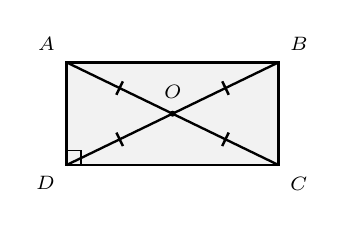
\begin{tikzpicture}[scale=0.84, baseline={(0,1.35)}, every node/.style={font=\scriptsize}]
    \coordinate (D) at (0,0); \coordinate (C) at (3.20,0);
    \coordinate (A) at (0,1.55); \coordinate (B) at (3.20,1.55);
    \coordinate (O) at (1.60,0.775);
    \fill[gray!10] (A)--(B)--(C)--(D)--cycle;
    \draw[line width=0.95pt] (A)--(B)--(C)--(D)--cycle;
    \draw[line width=0.85pt, tk1] (A)--(O); \draw[line width=0.85pt, tk1] (O)--(D);
    \draw[line width=0.85pt, tk1] (B)--(O); \draw[line width=0.85pt, tk1] (O)--(C);
    \draw[line width=0.65pt] (0,0.22)--(0.22,0.22)--(0.22,0);
    \fill (O) circle (1.3pt) node[above=2pt] {$O$};
    \node[above left=1pt] at (A) {$A$}; \node[above right=1pt] at (B) {$B$};
    \node[below right=1pt] at (C) {$C$}; \node[below left=1pt] at (D) {$D$};
  \end{tikzpicture}
\end{tabular}

\vspace{4pt}
\begin{tcolorbox}[enhanced, sharp corners, colback=panelgray, colframe=black, boxrule=0.8pt, top=4pt, bottom=4pt, left=6pt, right=6pt]
  \textbf{ខ. សំណួរត្រួតពិនិត្យរហ័ស (\en{Exit Check} — គូសរង្វង់ចម្លើយត្រឹមត្រូវតែ ១)៖}\par
  ក្នុងចតុកោណកែង $ABCD$ (ផ្ចិត $O$) បើ $AC = 12\unit{cm}$ និង $\ang{OAB} = 55^\circ$ តើប្រវែង $OB$ និងរង្វាស់មុំ $\ang{OAD}$ ស្មើប៉ុន្មាន?\par\vspace{2pt}
  \hspace*{0.2cm}\textbf{A.} $OB=12\unit{cm}, 45^\circ$ \hspace{0.9cm} \textbf{B.} $OB=6\unit{cm}, 35^\circ$ \hspace{0.9cm} \textbf{C.} $OB=6\unit{cm}, 45^\circ$ \hspace{0.9cm} \textbf{D.} $OB=6\unit{cm}, 55^\circ$
\end{tcolorbox}

% --- Step 5 Homework ---
\secbar{ផ្នែកទី៦ ៖ កិច្ចការផ្ទះ និងបណ្ដាំផ្ញើ \enbf{(}ទំព័រ ១៧៤--១៧៦ និង ១៨៦\enbf{)}}{ធ្វើក្នុងសៀវភៅកិច្ចការផ្ទះ}
$\bullet$ \textbf{លំហាត់ទី១ (ពង្រីកពីលំហាត់ទី៩ ទំព័រ ១៨៦)៖} ក្នុងចតុកោណកែង $ABCE$ (ផ្ចិត $F$) និងប្រលេឡូក្រាម $BCDE$ បើ $BF = 5\unit{cm}$ ចូរគណនាប្រវែង $BE, AC$ និង $CD$ ព្រមទាំងបញ្ជាក់ប្រភេទនៃត្រីកោណ $ACD$ ។\par\vspace{2pt}
$\bullet$ \textbf{លំហាត់ទី២៖} ក្នុងប្រលេឡូក្រាម $ABCD$ អង្កត់ទ្រូងកាត់គ្នាត្រង់ $O$ ដោយ $OA = 2x + 1\unit{cm}$, $OC = 7\unit{cm}$ និង $BD = 14\unit{cm}$ ។ រកតម្លៃ $x$ រួចបញ្ជាក់ថា $ABCD$ ជាចតុកោណកែង ហើយអានជាមុន \textbf{២.៣ លក្ខណៈចតុកោណស្មើ} (ទំ.១៧៦--១៧៩) ។

\end{document}
